\documentclass[10pt]{article}
\usepackage{graphicx,amssymb, amstext, amsmath, epstopdf, booktabs, verbatim, gensymb, geometry, appendix, natbib, lmodern, hyperref}
\geometry{letterpaper}
%\usepackage{garamond}

\newcommand*\Title{Neurowrx Account Manual}
\newcommand*\cpiType{some subtitle}
\newcommand*\Date{Novermber 2018}
\newcommand*\Author{Michael Braeutigam}
\title{Neurowrx Account Manual}
\author{Michael Braeutigam}
\date{\today}
%-----------------------------------------------------------

\usepackage{cpistuff/cpi} % This is what makes your document look like a cpi document.


\begin{document}

\begin{titlepage}
\maketitle
\end{titlepage}

\linespread{1.15} %Set standard document linespacing

\begin{executive}

This is a document describing the fuctionality of the neurowrx website.

\frame{
\textbf{Important Title}

Something should be said in here to the effect of "you shouldn't use the information contained in here maliciously", blahdiblah.}
\end{executive}

\tableofcontents









%\subsection{green writing}

%Use the \texttt{callout} command:

%\callout{By the shores of gitchee gumee\\ by the shining big sea waters \\ stood the wigwam of Nokomis \\ brother of the moon, Nokomis.}



%Use the \texttt{frame} command:

%\frame{ 'Twas brillig and the slithy toves did gyre and gimble in the wabe \\ all mimsy were the borogroves, and the mome raths outgrabe. \\ Beware the Jabberwock, my son, the claws that bite, the jaws that snatch \\ Beware the Jubjub bird, and shun the frumious Bandersnatch.}

%\ref{accountemail} returns the index of the figure in the document


\section{Ordinary Members}

\subsection{Account Creation}

\begin{flushleft}
Once you are a neurowrx member, a username (probably based on your actual name, or organization name) will be chosed by the site admin, and you will receive an email at the address that you provided in your application.  It will have neurowrx in the subject line so check your spam filter if you do not recieve it promptly.  It will notify you of your username and give you a link to a page where you can set your password, as well as a link to the regular login panel.  The login panel can be reached though this link or though the main site at \url{https://neurowrx.org/}, by clicking on the button at the top right corner. 
\end{flushleft}

\begin{figure}[h]
\centering
\caption{A typical account creation email}
\label{accountemail}
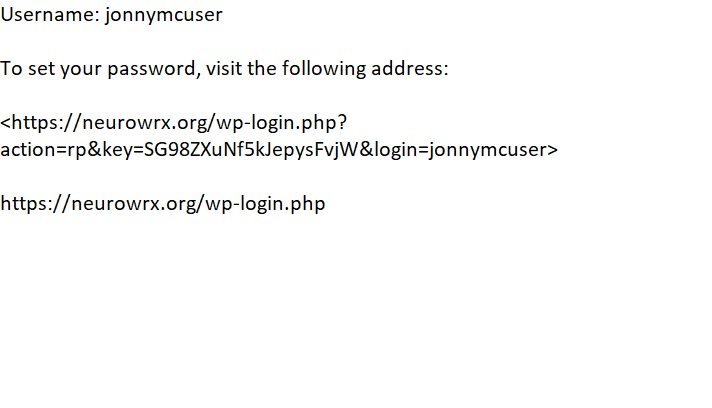
\includegraphics[scale=1.0]{images/accountcreation.jpg}
\end{figure}

The account's password is initially randomized and should be set via the first link before one attempts to log in.  In the case that the password is forgotten, it can be recovered though a link on the main login page at \url{https://neurowrx.org/wp-login.php}.

\begin{figure}[h]
    \centering
    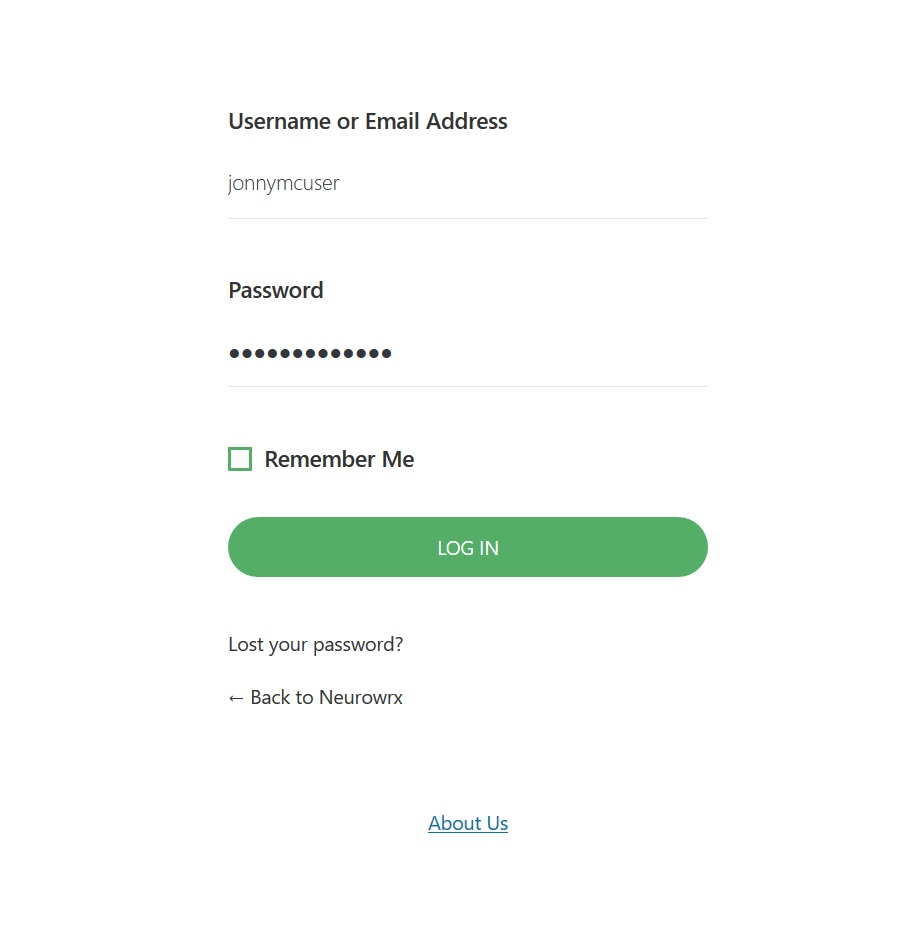
\includegraphics[scale=0.3]{images/loginpage.jpg}
    \caption{The login page}
    \label{loginpage}
\end{figure}

\begin{flushleft}
After you have chosen your password, you can log in with either your username, or with your email address.  Both are required to be unique, and in the case that you have more than one account; you must provide distinct email addresses for distinct accounts. 
\end{flushleft}

\begin{flushleft}
Once a successful login has occured, the top panel of the website changes to give the user access to the communication features.  A link for the members section appears, as well as an icon for private messages, notifications, and another for settings.  There is also a menu hiding under the profile picture with more features which will be discussed in succeeding sections. 
\end{flushleft}

\begin{figure}[h]
    \centering
    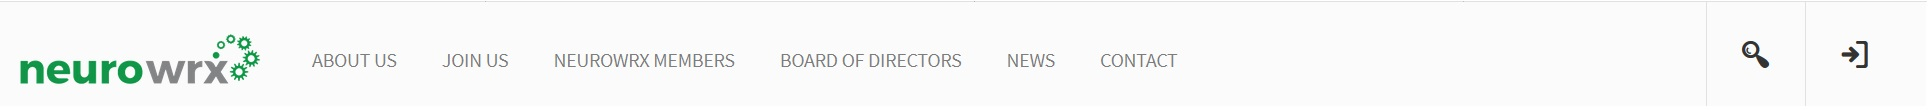
\includegraphics[scale=0.3]{images/topbar.jpg}
    \caption{The top panel that is publicly visible}
    \label{topbar}
\end{figure}

\begin{figure}[h]
    \centering
    
\includegraphics[scale=0.3]{images/topbarlogged.jpg}
    \caption{The top panel after login}
    \label{topbarlogged}
\end{figure}

\subsection{Profile Editing}

\begin{flushleft}
By hovering the mouse over the profile pic, a dropdown menu (with association submenus) becomes available.   
\end{flushleft}




\subsection{Messenging}
\subsection{Joining Groups}
\subsection{Uploading Documents}

\section{Group Moderators}
\section{Administrators}


\bibliography{codes_impact}
\bibliographystyle{plainnat}

\end{document}